\chapter{Tổng quan tiến hóa đa nhiệm}
\label{chap:introduction}
Chương này sẽ giới thiệu khái niệm cơ bản về thuật toán tiến hóa trong việc giải quyết các bài toán tối ưu. Cùng với đó là các thành phần, cơ chế hoạt động của thuật toán tiến hóa đa nhiệm, tiến hóa đa nhiệm với ước lượng hệ số trao đổi trực tuyến sẽ được giải thích.
\section{Giải thuật tiến hóa}
\subsection{Giới thiệu}
\label{section:cea}
Thuật toán tiến hóa (thuật ngữ gốc: \emph{Evolutionary Algorithm - EA})\cite{jansen2015analyzing} là tập các thuật toán được lấy cảm hứng từ ý tưởng tiến hóa \cite{darwin1859on} trong sinh học mà có thể đã khá quen thuộc với chúng ta đó là quá trình chọn lọc tự nhiên. Trong tiến hóa tự nhiên, một quần thể sẽ truyền lại những đặc tính di truyền của mình phù hợp với điều kiện sống hiện tại cho thế hệ sau. Những đặc tính này sẽ được biểu hiện và truyền lại trên gen từ bố mẹ sang con cái thông qua quá trình sinh sản. Trong đó việc các cá thể của thế hệ sau có đặc tính khác nhau là kết quả của quá trình "đột biến", "tái tổ hợp di truyền" và các "biến dị di truyền" khác. Trong quần thể, nếu một cá thể có nhiều đặc tính tốt phù hợp để sống sót với điều kiện sống nó sẽ có nhiều cơ hội để kết hợp sinh sản với các cá thể ưu tú khác trong quần thể để tạo ra những đứa con chất lượng trong thế hệ tiếp theo. Những cá thể yếu hơn và gen của chúng do không phù hợp với môi trường sống dần sẽ bị đào thải và biến mất. 

Việc mô phỏng quá trình tiến hóa tự nhiên này để phát triển một thuật toán chung nhằm dần cải thiện một cấu hình, một bộ tham số cho bất kỳ bài toán, giải pháp nào. Thuật toán bao gồm 4 bước chính như trong hình \ref{fig:ea}: khởi tạo quần thể, lựa chọn, toán tử di truyền và kết thúc. Mỗi bước sẽ tương ứng, đại khái một khía cạnh cụ thể của chọn lọc tự nhiên.

% \begin{figure}
%     \centering
%     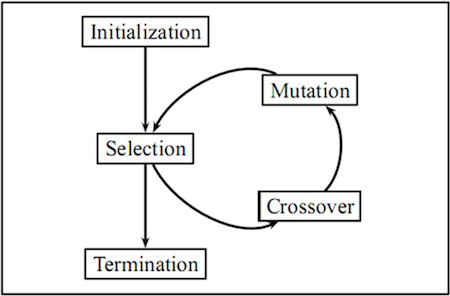
\includegraphics[width=7cm]{ea_process.jpeg}
%     \caption{Quá trình thực hiện thuật toán tiến hóa}
%     \label{fig:ea-process}
% \end{figure}

Tại mỗi thế hệ thuật toán sẽ cố gắng đưa ra một quần thể các giải pháp có chất lượng cao hơn số với thế hệ trước đó. Trong quá trình này, thuật toán sẽ thực hiện tính toán theo một thang đo phù hợp để tìm ra những cá thể có chất lượng tốt, kết hợp chúng để sinh sản ra con cái với chất lượng cao hơn tại thế hệ sau. Bởi vậy có thể coi những cá thể của thế hệ sau mang những vật liệu di truyền (gen) tốt nhất của thế hệ trước và vượt trội hơn một chút so với thế hệ trước. Hay nói một cách đơn giản, trong thuật toán tiến hóa các cá thể phù hợp sẽ tồn tại và sinh sôi nảy nở, ngược lại những cá thể yếu hơn sẽ chết đi và không đóng góp vào nhóm gen của thế hệ tiếp theo.




\subsection{Tối ưu hóa liên tục}
\subsubsection{Tổng quan}
Trong toán học và khoa học máy tính, bài toán tối ưu hóa là bài toán tìm kiếm lời giải tốt nhất trong tập tất cả các lời giải khả thi. Tối ưu hóa liên tục là một nhánh của tối ưu hóa cùng với tối ưu hóa rời rạc. Điểm khác nhau giữa chúng duy nhất ở không gian biến quyết định là liên tục hoặc rời rạc.

Về mặt toán học, tối ưu hóa liên tục là cực tiểu hóa (thuật ngữ gốc: \textit{minimization}) hoặc cực đại hóa (thuật ngữ gốc: \textit{maximization}) một hàm liên tục sao cho thỏa mãn được các ràng buộc của bài toán. Trên thực tế, bài toán cực tiểu hóa hay cực đại hóa có thể dễ dàng biến đổi qua lại bằng các phép toán học đơn giản. Do vậy, không mất tính tổng quát, kể từ đây đến hết đồ án, khi đề cập đến thuật ngữ tối ưu hóa mà không có giải thích bổ sung thì sẽ ngầm định nói về bài toán cực tiểu hóa.

\subsubsection{Bài toán tối ưu hóa liên tục}
\begin{definition}
    Bài toán tối ưu hóa liên tục: cực tiểu hóa hàm $f(x), x\in \mathbb{R}^n$ ký hiệu là $\min_{x \in \mathbb{R}^n} f(x)$ sao cho $g_i(x) \leq 0$ với $i = 1,...p$ và $h_i(x) = 0$ với $i = 1,....q$ trong đó:
    \begin{itemize}
        \item $x \in \mathbb{R}^n$ là biến quyết định
        \item $f(x): \mathbb{R}^n \rightarrow \mathbb{R}$ là hàm mục tiêu
        \item $g_i(x) \leq 0$ là các ràng buộc bất đẳng thức
        \item $h_i(x) = 0$ là các rằng buộc đẳng thức
    \end{itemize}
\end{definition}
    Lời giải của bài toán là nghiệm $x^* \in \mathbb{R}^n$ thỏa mãn $g_i(x^*) \leq 0, h_i(x^*) = 0$ và $f(x^*) <= f(x) \forall x \in \mathbb{R}^n$. Trong trường hợp $p = q = 0$ thì ta gọi đó là bài toán tối ưu hóa liên tục không ràng buộc. Trường hợp hàm $f(x)$ là hàm lồi, tức là thỏa mãn điều kiện:
    \begin{center}
    $f(\alpha x_1 + \beta x_2) \leq \alpha f(x_1) + \beta f(x_2); \forall x_1,x_2 \in \mathbb{R}^n; \forall \alpha \geq 0, \beta \geq 0, \alpha + \beta = 1,$
    \end{center} thì ta gọi đó là bài toán \textit{tối ưu lồi}.
    
    Các phương pháp giải quyết bài toán tối ưu hóa liên tục không có ràng buộc
    ở dạng tổng quát thường hướng đến coi bài toán ở dạng tìm kiếm hơn là đưa ra
    một công thức tường minh. Điểm chung của các thuật toán đều xuất phát từ một lời giải $x_0$, sau đó thực hiện các chiến lược nhất định để cập nhật $x_1, x_2, ...x_k$ cho tới khi tìm được giá trị $f$ tốt nhất có thể. 
    Các giải thuật chủ yếu khác nhau
    về cách thức xây dựng chiến lược cập nhật lời giải từ những lời giải đã duyệt qua. Một số phương pháp thường được sử dụng như sau:
    \begin{itemize}
        \item \textbf{Phương pháp đường tìm kiếm}: Lựa chọn một hướng tìm kiếm cố định sau đó cập nhật lời giải ở mỗi bước lặp tìm kiếm. Ví dụ thuật toán gradient descent.
        \item \textbf{Phương pháp heuristic}: Là các kỹ thuật dựa trên kinh nghiệm để giải quyết vấn đề, học hỏi hay khám phá nhằm đưa ra một giải pháp mà không được đảm bảo là tối ưu. Các phương pháp heuristic được sử dụng rộng rãi trong các bài toán tối ưu hóa liên tục bởi tính đơn giản và hiệu quả của chúng trong việc tìm ra một lời giải khả thi trong khoảng thời gian chấp nhận được. Ví dụ giải thuật tìm kiếm địa phương (thuật ngữ gốc: \emph{local search}), EA.
    \end{itemize}
    Trong đồ án này sẽ xem xét phương pháp heuristic để giải quyết bài toán tối ưu hóa liên tục mà cụ thể là sử dụng giải thuật tiến hóa. 
% Từ những đặc điểm được mô tả trong phần 1.1.1, EA phù hợp với việc tìm giải pháp cực trị, có thể là tối thiểu hóa hoặc tối đa hóa. Loại bài toán này có thể được mô tả dưới dạng là một \emph{bài toán tối ưu}\cite{boyd2004cvx}. Không mất tính tổng quát, nó có dạng:
% \begin{equation}
%     \begin{array}{ll}{\text { Tối đa hàm }} & {f_{0}(x)} \\ {\text { Với điều kiện }} & {f_{i}(x) \leq b_{i}, \quad i=1, \ldots, m}\end{array}
% \end{equation}
% trong đó 
% \begin{itemize}
%     \item $x$ là \emph{giá trị tối ưu} của bài toán. Sao cho $x \in S$ với $S$ là tập các giải pháp phù hợp. $S$ có thể bao gồm hoặc tập giá trị nhị phân $\{0, 1\} ^ n$, tổ hợp rời rạc $\{1,2,...,k\}^n$ hoặc các giá trị liên tục thuộc $\mathbf{R} ^ n$.
%     \item Hàm số $f_0: S \rightarrow \mathbf{R}$ được gọi là \emph{hàm mục tiêu}.
%     \item Hàm số $f_{i} : \mathbf{R}^{n} \rightarrow \mathbf{R}, \; i=1, \ldots, m$ là \emph{bất đẳng thức ràng buộc} với các giá trị biên $b_{1}, \dots, b_{m}$
% \end{itemize}\\
% \emph{Bài toán tối ưu} nhằm mục tiêu tìm kiếm một \emph{giải pháp tối ưu} cho giá trị hàm mục tiêu nhỏ nhất trên tất cả các véc-tơ thảo mãn ràng buộc.
% Giải pháp này được ký hiệu là $x*$.\\
% Trong đồ án này, tôi sẽ tập trung xem xét bài toán tối ưu hóa trên miền liên tục không có ràng buộc, sau đây gọi là \emph{tối ưu hóa liên tục}. Có nhiều nhóm thuật toán để giải quyết bài toán \emph{tối ưu hóa liên tục}, trong đó có thể kể đến phương pháp phân tích như tối ưu hóa hàm lồi (convex optimization)\cite{boyd2004cvx}. Vì EA xem xét vấn đề giống như một bài toán hộp đen (black-box problem) nên cụ thể EA sẽ giải quyết vấn đề bằng cách sử dụng thông tin của hàm mục tiêu mà không sử dụng thông tin về cấu trúc của vấn đề. \\
% Mục tiếp theo tôi sẽ giải thích quá trình thực hiện của EA và các thành phần cơ bản trong việc giải quyết vấn đề \emph{tối ưu hóa liên tục}.
\subsection{Giải thuật tiến hóa cho tối ưu hóa liên tục}
\label{subsection:ea-continuous}
Giải thuật tiến hóa - hay còn gọi là EA là một thuật toán được xây dựng dựa trên quần thể và quần thể là tập hợp của những giải pháp khả thi. Trong ngữ cảnh của tối ưu hóa liên tục, EA duy trì quần thể của các vector tốt nhất. Quần thể sẽ thay đổi từ thời điểm này đến thời điểm khác, chúng ta gọi tập hợp tại một lần thay đổi là một thế hệ. Việc lựa chọn quần thể thế hệ đầu tiên được gọi là quá trình khởi tạo. Trong mọi thế hệ, mỗi cá thể trong quần thể sẽ được đánh giá dựa trên độ thích nghi (thuật ngữ gốc: \emph{fitness}) của nó. Những cá thể ưu tú, có độ thích nghi cao được lựa chọn, kết hợp lại với nhau và sản sinh ra thế hệ con cháu. Những cá thể được lựa chọn này sẽ được gọi là quần thể cha mẹ. Quần thể cha mẹ và quần thể con cháu kết hợp với nhau tạo ra một tập cá thể mới. Sau đó sẽ tiếp tục lựa chọn những cá thế tốt nhất trong đó để lập thành quần thể cho thế hệ tiếp theo. Quá trình chọn lọc đó cứ lặp đi lặp lại, cho đến khi điều kiện kết thúc được thỏa mãn: ví dụ khi giải pháp tốt nhất thu được tại một thế hệ có giá trị lớn hơn một giá trị cho trước nào đó hoặc số thế hệ tiến hóa đạt giá trị tối đa.

Thuật toán tiến hóa khi kết thúc sẽ trả về giải pháp tốt nhất thu được. Nói chung EA là một thuật toán tối ưu hóa tương đối đơn giản để thực hiện và phù hợp với hầu hết các loại bài toán tối ưu. Mặc dù vậy giải pháp tối ưu được tìm ra bởi EA không được đảm bảo chắc chắn là giải pháp tối ưu nhất (thuật ngữ gốc: \emph{optimal solution}), tuy nhiên đây lại là một giải pháp gần đúng nhất có thể tìm được trong một khoảng thời gian hợp lý.
\begin{figure}[ht]
    \centering
    \fbox{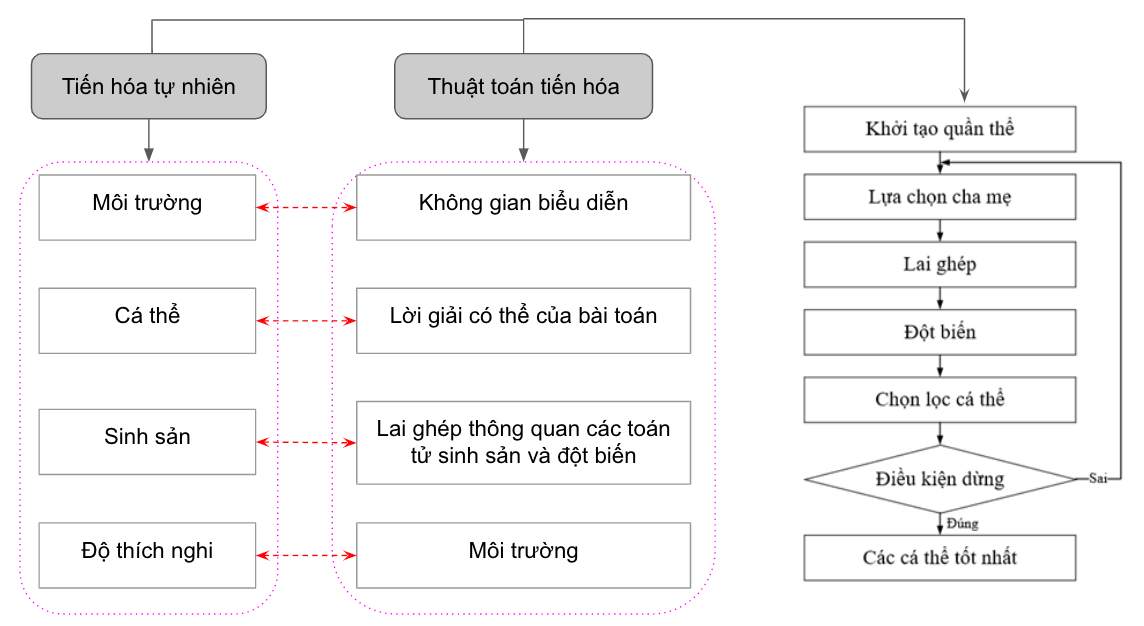
\includegraphics[width=0.85\linewidth]{ea_.png}}
    \caption{Tổng quan và các bước trong thuật toán tiến hóa}
    \label{fig:ea}
\end{figure}
\subsubsection{Khởi tạo}
 Quá trình khởi tạo - hay còn gọi là quá trình \textit{initialization} là quá trình khởi tạo một quần thể cho thế hệ đầu tiên. Đối với các bài toán tối ưu hóa liên tục, việc khởi tạo hầu hết được thực hiện theo cách ngẫu nhiên, chọn giá trị cho véc-tơ giải pháp trên một không gian nghiệm giới hạn. Với nhiều bài toán, thay vì lựa chọn một cách ngẫu nhiên, ta có thể dựa vào kết quả của một thuật toán tối ưu khác dựa vào một vài tri thức đã biết hoặc kinh nghiệm. Cách làm này có thể làm tăng tốc EA nhưng nó cũng là nguyên nhân gây ra sự đa dạng hóa thấp đi của lời giải vì quần thể được chọn đã rất giống lời giải so với lần chạy thực nghiệm trong thuật toán trước.
 Cách tiếp cận tốt nhất trong việc đưa ra quần thể đầu tiên có lẽ là nên nghiên cứu kỹ về các thuộc tính của vấn đề cần giải quyết bởi EA, sau đó chọn những thuộc tính mà ta quan tâm. Ví dụ, quần thể với mạng neural nhân tạo (thuật ngữ gốc: \emph{Artificial Neural Network - ANN}) có thể được khởi tạo bởi sơ đồ glorot ngẫu nhiên. \cite{glorot2010understanding}
 \subsubsection{Lựa chọn}
 Quá trình lựa chọn hay quá trình \emph{selection} có 2 kiểu khác nhau được thực hiện xuyên suốt trong mọi thế hệ đó là: lựa chọn để sinh sản và lựa chọn để thay thế trong quần thể. Lựa chọn để sinh sản được lấy cảm hứng từ tiến hóa trong sinh học, khi chỉ có những cá thể tốt nhất, khả năng sống sót cao nhất mới có thể truyền những yếu tố, đặc tính trong vật liệu di truyền của nó đến thế hệ con cháu. Giống như vậy, quy trình lựa chọn thay thế cũng giống như thực tế khi chỉ có những con cái khỏe mạnh với những đặc điểm tốt được thừa hưởng bởi bố mẹ mới có thể sống sót đến thế hệ tiếp theo. 
%  Nhưng thế nào là cá thể có đặc tính tốt, có khả năng sống sót cao? Tùy vào mỗi trường hợp khác nhau, yếu tố này sẽ thay đổi tuy nhiên dưới đây tôi xin trình bày một số phương pháp \emph{lựa chọn} trực tiếp liên quan đến đồ án này:
 
%  \begin{enumerate}
%  \item \textbf{Uniform selection:} Một cá thể được lựa chọn một cách ngẫu nhiên. Đây là hình thức chọn lọc yếu nhất vì không có điều kiện chọn lọc gì, áp lực chọn lọc thấp. Ngay cả những cá thể yếu nhất vẫn có những cơ hội bình đẳng được lựa chọn để tái sản xuất và di truyền đặc tính đến thế hệ tiếp theo so với những cá thể tốt nhất. Đây là một ví dụ dựa trên cách chọn lọc bình đẳng tuy nhiên cách này hầu như không được sử dụng.
%  \item \textbf{Fitness-proportional selection:} Giả sử rằng tất cả những giá trị fitness của hàm mục tiêu có giá trị dương. Một cá thể $x$ trong quần thể của thế hệ hiện tại $P$ có thể được chọn với xác suất $\frac{f(x)}{\sum_{u \in P}{f(u)}}$. Thay vì lựa chọn ngẫu nhiên như phương pháp \emph{uniform selection}, hình thức nãy sẽ đặt ra một độ đo để thực hiện chọn lọc. Tuy nhiên cách tiếp cận này lại phụ thuộc lớn vào những giá trị tốt fitness của hàm mục tiêu. Ví dụ: Nếu sự khác biệt giữa giá trị fitness trong dân số là quá lớn thì các cá thể có fitness cao nhất sẽ luôn được ưu tiên lựa chọn. Điều này sẽ làm ảnh hưởng đến sự đa dạng của quần thể hiện tại, và dẫn đến EA không thể khám phá ra khu vực thiết yếu trong không gian tìm kiếm. Tuy nhiên nếu các giá trị fitness của các cá thể là tương đương thì phương pháp này sẽ trở nên tương tự phương pháp \emph{uniform selection}. Thông thường trong những thế hệ đầu của EA trong việc giải quyết bài toán tối ưu hóa liên tục, giá trị fitness còn thấp nên sự khác biệt lớn giữa các cá thể sẽ mang tính quyết định. Các thế hệ sau đó, khi giá trị fitness của từng cá thể trong quần thể cao hơn, sự chênh lệch giữa chúng giảm dần, cơ chế lựa chọn sẽ dần trở thành tương tự \emph{uniform selection}. Hiện tượng này sẽ dần đến giảm hiệu quả trong quá trình lựa chọn và để giải quyết vấn đề này tôi sẽ giới thiệu phương pháp \emph{rank selection} như dưới đây.
%  \item \textbf{Rank selection:} Thay vì trực tiếp sử dụng fitness, kĩ thuật này sẽ thực hiện sắp xếp rank theo thứ tự giảm dần của fitness. Bằng phương pháp này, việc phụ thuộc vào những giá trị cụ thể của fitness bị loại bỏ. Việc lặp lại quá trình của \emph{fitness-proportional selection} dẫn đến trở về quá trình \emph{uniform selection} sẽ không xảy ra. Phương pháp này thường xuyên được sử dụng, áp dụng. Đặc biệt là thuật toán tối ưu hóa đa nhiệm hiện đại cũng áp dụng \emph{rank selection} để làm cơ sở trong việc tạo áp lực chọn lọc trong quá trình cải tiến nhiều nhiệm vụ của mình.
%  \end{enumerate}
 
 \subsubsection{Lai ghép}
Quá trình lai ghép (thuật ngữ gốc: \emph{crossover}) nhằm mục đích lấy những đặc điểm tốt của 2 hay nhiều cá thể cha mẹ để tạo ra những cá thể con cái có chất lượng cao hơn, mang một phần đặc tính di truyền của bố mẹ. Con cái được sinh ra có một phần sẽ giống với bố mẹ chúng và có thể khai thác được những gì mà bố mẹ chúng đã biết. Đồ án sẽ giới thiệu một số cơ chế lai ghép liên quan đến phạm vi nghiên cứu:

\begin{enumerate}
    \item \textbf{One point crossover:} Đầu tiên 2 cá thể $p_1$ và $p_2$ trong quần thể cha mẹ được chọn. Sau đó ta sẽ chọn hệ số chia cắt index $i \in \{1, ..., n-1\}$, Sau đó 2 cha mẹ sẽ hoán đổi tại vị trí $i$ giống như trong hình \ref{fig:introduction:one_point}.
    \begin{figure}[ht]
        \centering
        \fbox{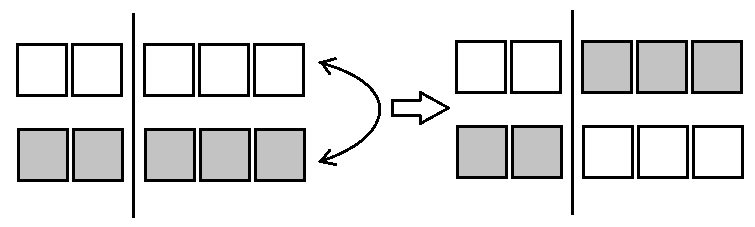
\includegraphics[width=0.8\linewidth]{images/one_point.png}}
        \caption{Kỹ thuật one point crossover}
        \label{fig:introduction:one_point}
    \end{figure}
    \item \textbf{Uniform crossover:} Đầu tiên 2 cá thể $p_1$ và $p_2$ trong quần thể cha mẹ được chọn. Sau đó với mỗi chiều $i \in \{1, ..., n\}$ giá trị của con cái $x_i$ sẽ là bản được sao chép từ một trong các cha mẹ của chúng. Quyết định cha mẹ nào sẽ được chọn để sao chép sẽ được tạo ra độc lập bởi tại mỗi chiều với xác suất bằng $\frac{1}{2}$.
    \item \textbf{Simulated binary crossover - SBX:} SBX \cite{deb1995simulated} \cite{deb94simulated} là một kỹ thuật lai ghép kết hợp tham số là số thực thường được sử dụng trong EA. Trong đó, một lời giải bao gồm các giá trị số thực liên tục cần được chuyển sang dạng nhị phân để áp dụng kĩ thuật one point crossover với các lời giải khác. Tuy nhiên thay vì sử dụng cách này, SBX được thiết kế để chỉ sử dụng các phân phối xác suất. Các bước của SBX được mô tả như dưới đây:
        \begin{enumerate}
            \item Chọn cặp bố mẹ $p_1$ và $p_2$ để lai ghép ($p_1, p_2 \in \text{ khoảng } [0, 1] ^ n$)
            \item Khởi tạo ngẫu nhiên véc-tơ $u \sim U(0,1)^n$
            \item Khởi tạo đặc tính chung $cf$
                 \[
                    cf=\left\{
                        \begin{array}{ll}
                            2*u_i^{\frac{1}{\alpha + 1}} \text{ if } u_i > 0.5\\
                            2*(1-u_i)^{\frac{-1}{\alpha + 1}} \text{ if } u_i \leq 0.5\\
                        \end{array}
                    \right.
                  \]
                Tham số $\alpha$ là chỉ số của phân phối SBX, thường có giá trị từ $2$ đến $5$. Hình \ref{fig:introduction:sbx} biểu thị mối quan hệ giữa của tập con cái và cha mẹ khi được sinh ra bởi các phân phối SBX khác nhau. Chỉ số phân phối nhỏ hơn sẽ khuyến khích sự khám phá vì con cái tương đối xa cha mẹ của chúng.
            \item Tạo 2 con
                 \[
                     \begin{array}{ll}
                        c_1 = \frac{1}{2} (1 + cf) * p_1 + (1 - cf) * p_2\\
                        c_2 = \frac{1}{2} (1 + cf) * p_2 + (1 - cf) * p_1
                    \end{array}
                  \]
        \end{enumerate}
        \begin{figure}[ht]
            \centering
            \fbox{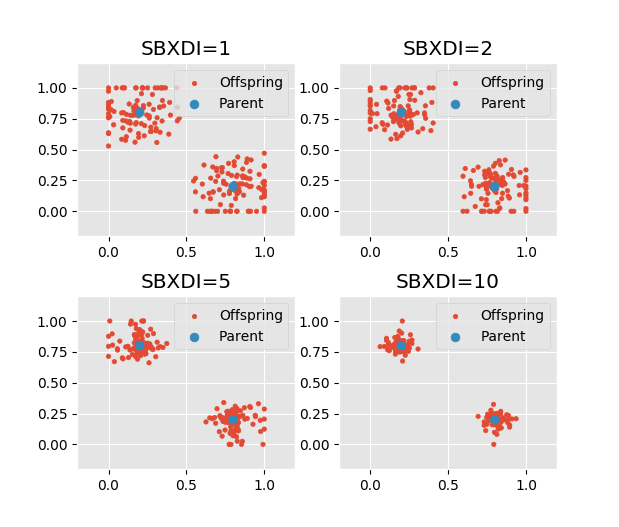
\includegraphics[width=0.8\linewidth]{sbx.png}}
            \caption{Mô phỏng 100 con cái được tạo ra từ thuật toán lai ghép SBX với các chỉ số phân phối khác nhau}
            \label{fig:introduction:sbx}
        \end{figure}
\end{enumerate}

\subsubsection{Đột biến}
Ngược lại với lai ghép, mục đích của đột biến hay còn gọi là \emph{mutation} là để khám phá ra thêm không gian tìm kiếm. lai ghép khai thác, tái sử dụng những giá trị, thông tin đã tồn tại trong một tập các cá thể, bởi vậy quần thể được sinh ra sẽ ngày càng có độ đa dạng giảm đi. Do đó đột biến sẽ tạo ra những thay đổi nhỏ trong các giải pháp thu được, có thể hiểu một cách đơn giản như ta sẽ đưa thêm các vật liệu di truyền mới vào các nhóm gen đã có để tăng sự đa dạng của quần thể. Đột biến sẽ không tạo ra thay đổi lớn trong cá thể gốc bởi vì nó sẽ phá vỡ cấu trúc đã được hình thành trong giải pháp của quần thể cha mẹ, những con cái được chọn để đột biến là ngẫu nhiên mà không tuân theo nguyên tắc cụ thể nào.

Kết hợp quá trình lai ghép và đột biến sẽ giúp tinh chỉnh các tham số của lời giải nhằm mục đích cân bằng giữa việc khai thác và khám phá giúp EA tìm ra những giải pháp tối ưu hơn. Trong các phương pháp đột biến thì Gaussian mutation là một trong những kĩ thuật đột biến phổ biến nhất trong tối ưu hóa liên tục. Trong kĩ thuật này, các con cái là $y \in \mathbb{R}^n$ sẽ được xây dựng bằng cách sử dụng giải pháp của bố mẹ $x \in \mathbb{R} ^ n$ thêm với một lượng nhiễu nhỏ $m \in \mathbb{R}^n$. Giá trị nhiễu $m$ này sẽ phải đủ nhỏ để tuân theo nguyên tắc chỉ gây ra một chút thay đổi nhỏ cho tập con cái. Giá trị nhiễu $m \sim \mathbb{N}(0, I*\sigma^2)$ với $\sigma$ là độ lệch chuẩn nhỏ.
% \subsection{Các tham số của thuật toán tiến hóa}
% 
\subsubsection{Số chiều của không gian tìm kiếm $n$} Tham số này là số lượng tham số của bài toán. Ví dụ trong mmoojt bài toán tối ưu hóa liên tục có không gian tìm kiếm $x \in \mathbb{R}^n$. Sẽ có nhiều tham số khác phụ thuộc vào tham số $n$ này như xác suất cho đột biến xảy ra có thể tính dưới công thức $p_m=1/n$. Bên cạnh đó, số chiều của không gian tìm kiếm các lớn thì sẽ yêu cầu kích thước của quần thể $\mu$ lớn hơn, kích thước quần thể con cái $\lambda$ cũng lớn hơn.
    
\subsubsection{Kích thước quần thể $\mu$} Tham số này là số lượng cá thể trong quần thể. Nói chung thì không có quy tắc nào trong việc lựa chọn $\mu$ nhưng nếu $\mu$ quá nhỏ thì nhiều khả năng sẽ không thể giải quyết được bài toán. Nếu $\mu$ quá lớn thì thuật toán sẽ tốn rất nhiều chi phí tính toán.

\subsubsection{Kích thước quần thể con cái $\lambda$} Tham số này là số lượng cá thể mới được sinh ra trong mỗi thế hệ. 

\subsubsection{Tham số khác}
    \begin{itemize}
        \item Xác suất đột biến $p_m$
    \end{itemize}

\section{Tiến hóa đa nhiệm} 
% \subsection{Động lực của tiến hóa đa nhiệm}
% Với sự phát triển của EA các nhà nghiên cứu đã và đang tiếp tục đưa ra những hướng nghiên cứu mới, những thuật toán hiệu quả cao hơn. Trong những năm gần đây, \emph{tiến hóa đa nhiệm} nổi lên như là một xu hướng trong cộng đồng các nhà nghiên cứu \emph{thuật toán tiến hóa} và \emph{tính toán thông minh}. Không chỉ một mà nhiều bài toán tối ưu có thể được giải quyết cùng nhau, điều này còn được gọi với cái tên khác là \emph{tối ưu hóa đa tác vụ} (thuật ngữ gốc: \emph{multitask  optimization}.

Trong khoa học máy tính và học máy có một thuật ngữ được gọi là \emph{học đa nhiệm vụ } (thuật ngữ gốc: \emph{multitask learning}) nó khá tương đồng với \emph{multitask  optimization}. Trong \textbf{multitask learning} các tác vụ liên quan sẽ chia sẻ kiến thức với nhau, và được huấn luyện cách đồng thời. Lấy ví dụ trong hệ thống phân loại email rác, có thể coi đây là các tác vụ phân loại riêng biệt nhưng có liên quan giữa các người dùng với nhau. Cụ thể hơn, những người khác nhau sẽ có những cơ chế, đặc tính phân loại tin email và email thường khác nhau. Tuy nhiên, hầu hết người dùng đều không tự gán nhãn đủ để có thể xây dựng cơ chế đủ tốt phân loại email cá nhân hóa, trong khi dữ liệu lại quá nhiễu để sử dụng cơ chế phân loại chung cho tất cả các người dùng. Bởi vậy kỹ thuật \textbf{multitask learning} sẽ dựa vào thông tin từ những người dùng thường xuyên gán nhãn email để làm cơ sở kiến thức trong việc xây dựng cơ chế cá nhân hóa cho các người dùng khác. Trong khi đó, \textbf{multitask  optimization} cũng giúp các tác vụ được tối ưu một cách đồng thời nhưng là một thuật ngữ chung hơn, nó không phụ thuộc vào việc các thông tin trong mô hình được kết nối với nhau như thế nào để chia sẻ. Mà nó giúp giữa các tác vụ có liên quan đến nhau có thể chia sẻ không gian giải pháp với tác vụ khác để đẩy tốc độ tìm kiếm giải pháp tối ưu trên tác vụ đó, bao gồm cả các giải pháp rời rạc và tối ưu. 

Để cụ thể hơn, lấy ví dụ bài toán \emph{dịch vụ đám mây theo yêu cầu} (thuật ngữ gốc: \emph{cloud-based-on-demand}) cung cấp cho khách hàng sử dụng. Có thể hiểu là hệ thống sẽ phải giải quyết nhiều tác vụ tối ưu cùng lúc được nhận từ nhiều người dùng vào cùng một thời điểm. Mỗi tác vụ có thể có những đặc tính chung nào đó hoặc chúng hoàn toàn khác nhau. Nói một cách khác \textbf{multitask optimization} có thể được xem như là một mô thức chung trong việc giải quyết các bài toán tối ưu hóa. Không chỉ là việc chia sẻ kiến thức 1 chiều từ những tác vụ đơn giản đến tác vụ phức tạp, mà thực tế khi giải quyết những tác vụ phức tạp sẽ có thể giải quyết được những tác vụ đơn giản hơn. 

Một cách tiếp cận \empth{tiến hóa} cho \empth{multitask optimization} được gọi là \empth{evolutionary multitasking} hay còn gọi là tiến hóa đa tác vụ. Nó là một phương pháp kết hợp tư tưởng của thuật toán EA theo hướng tối ưu hóa nhiều vấn đề một cách đồng thời dựa theo cơ sở của lý thuyết \empth{multitask optimization}.
% \begin{figure}[ht]
%     \centering
%     \fbox{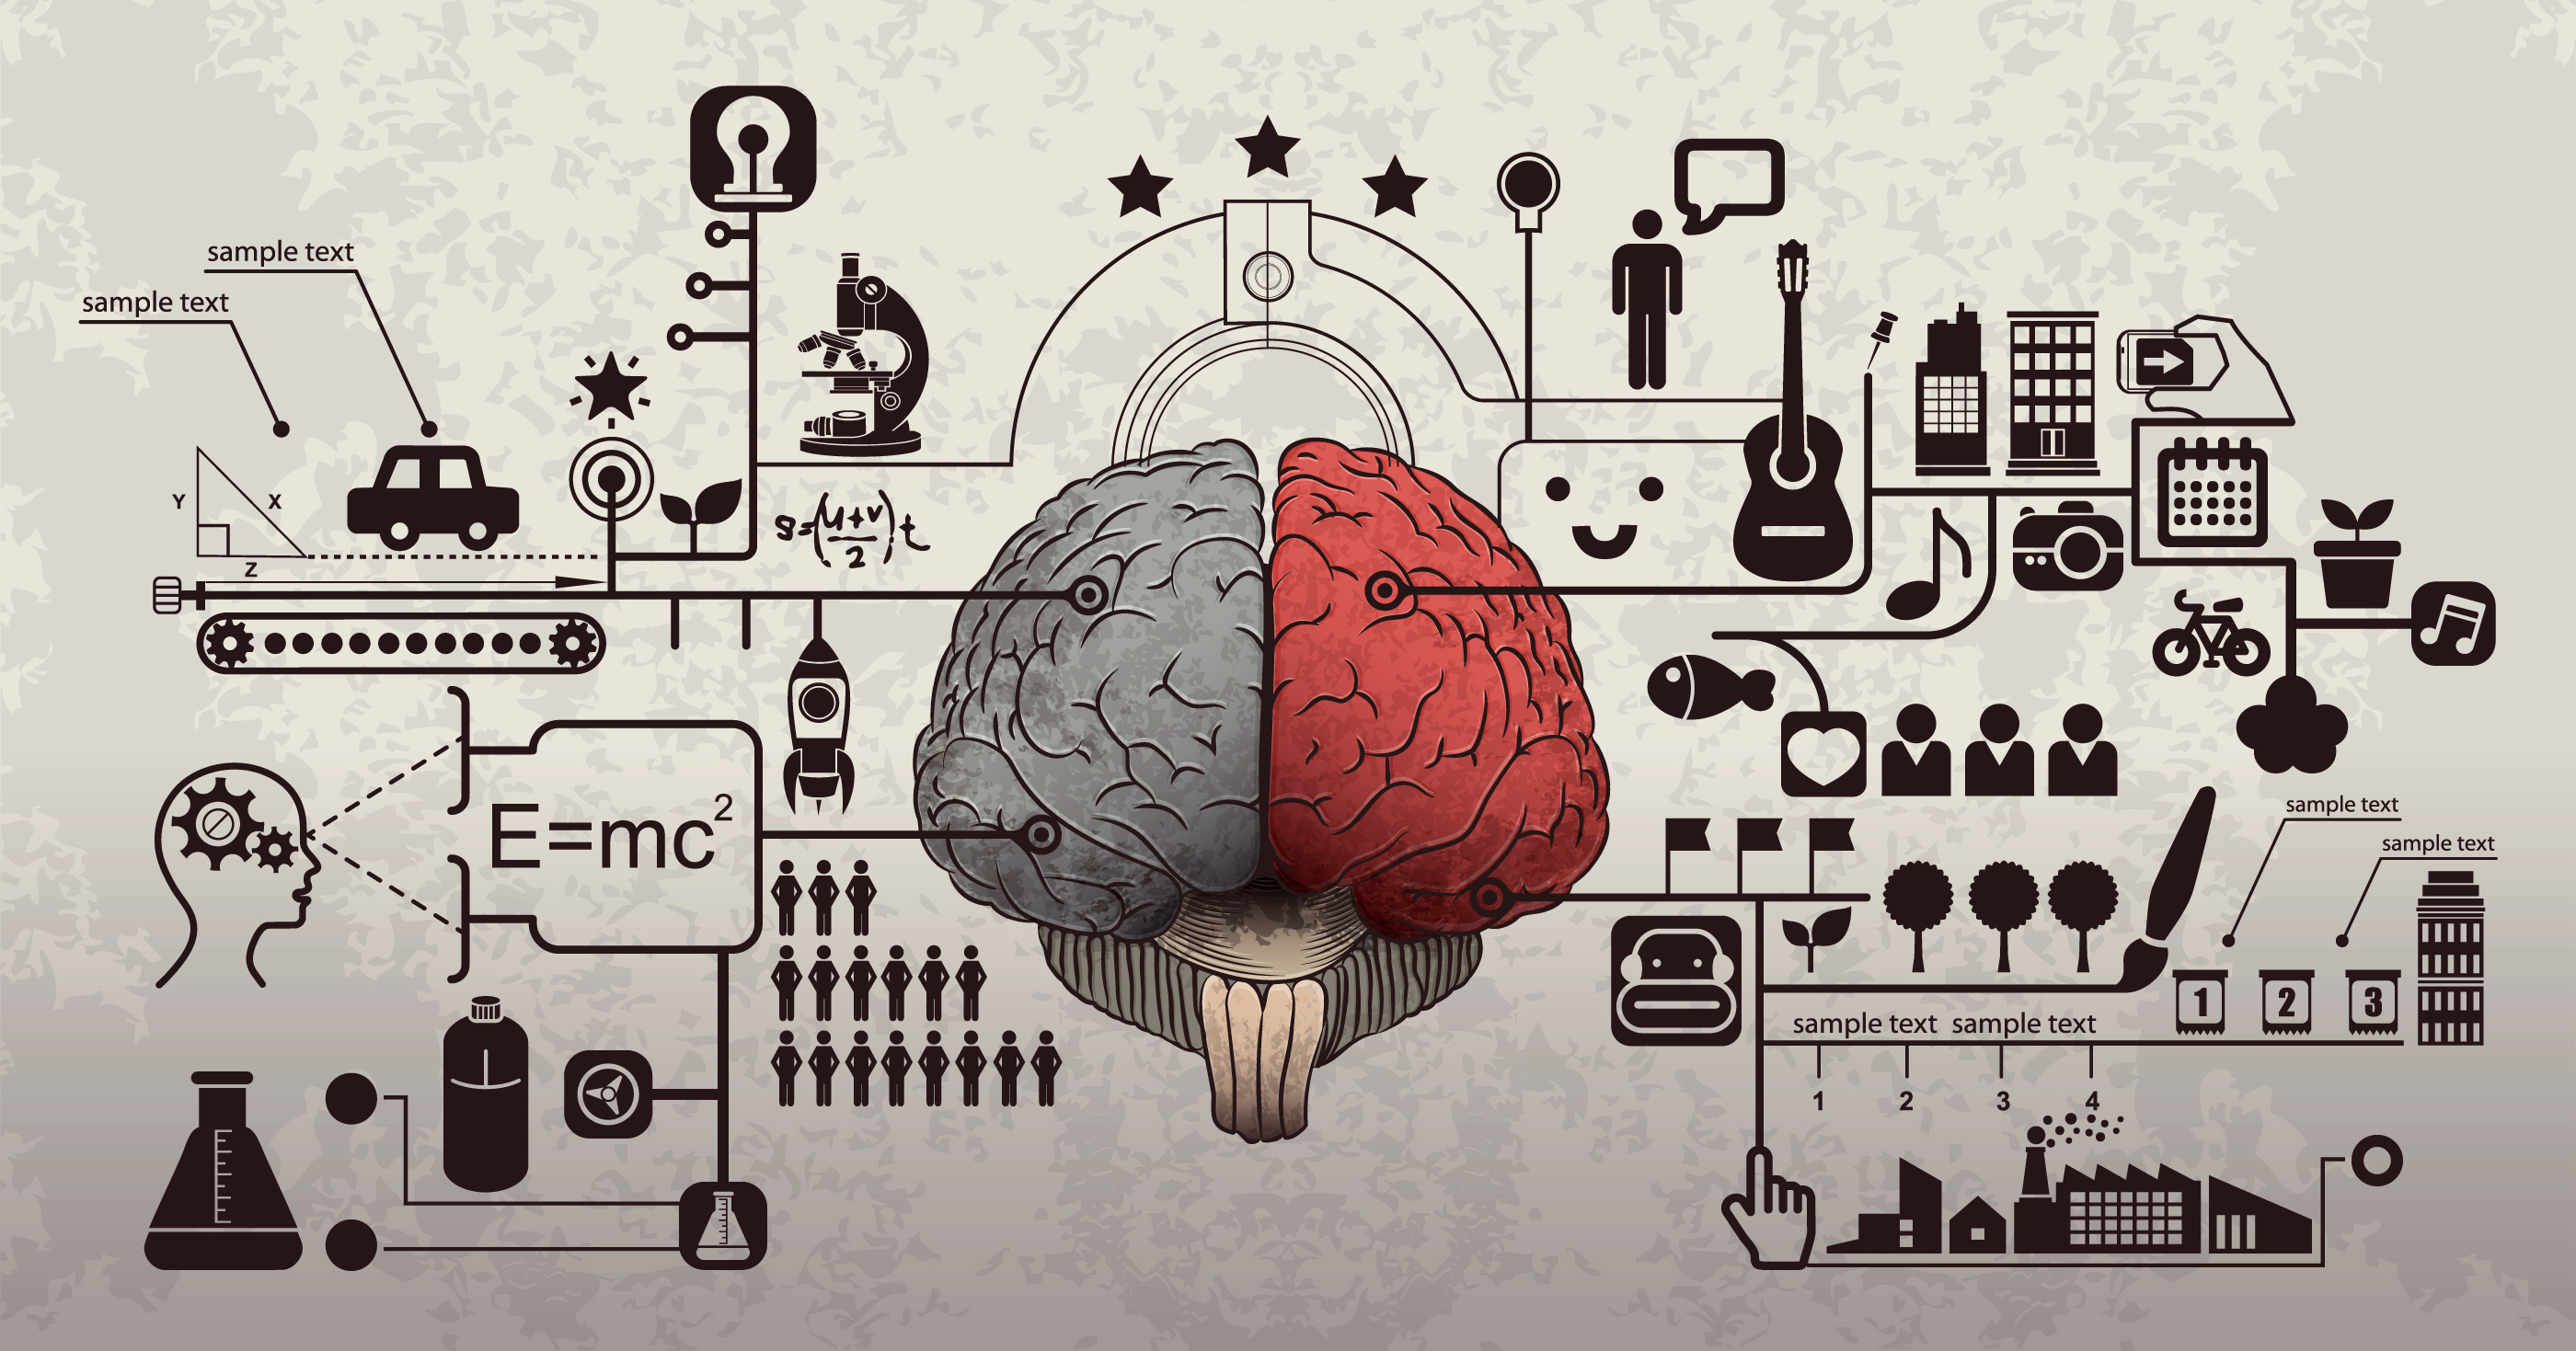
\includegraphics[width=0.6\linewidth]{mindfulness.jpg}}
%     \caption{Mô tả về đa nhiệm của nhận thức khi bộ não liên tục phải nhận nhiều tín hiệu từ các nguồn khác nhau và xử lý chúng đồng thời}
%     \label{fig:mfea:cognitive-multitasking}
% \end{figure}

Bên cạnh đó, tiến hóa đa nhiệm còn lấy cảm hứng ý tưởng từ tưởng, não của con người có thể giải quyết được nhiều tác vụ cùng một lúc. Lấy ví dụ, con người thường hay nói chuyện khi đi bộ, nghe nhạc khi đang học, vừa hát vừa đánh đàn vv.. các công việc này đều yêu cầu não bộ phải xử lý các thông tin khác nhau từ các tác vụ khác nhau. Một đứa trẻ khi lớn lên đã phải có khả năng giải quyết nhiều việc cùng một lúc, học nhiều môn học, học nhiều thứ tiếng. Việc giải quyết nhiều tác vụ cùng một lúc giờ đây là điều tất nhiên con người phải thích nghi để sống sót, tồn tại trong xã hội. So với trước đây, não bộ con người ngày càng được yêu cầu cao hơn, đòi hỏi phải xử lý nhiều thông tin hơn. Có một điểm cần lưu ý là tuy não bộ con người giải quyết nhiều tác vụ cùng một lúc, tuy nhiên khi chuyển từ tác vụ này sang tác vụ khác, nó có khả năng tái sử dụng những kinh nghiệm đã học được từ tác vụ trước đó để giải quyết tác vụ tiếp theo. 
\subsection{Tối ưu hóa đa nhiệm}
Trong những năm gần đây mô hình tối ưu đa nhiệm (thuật ngữ gốc: Multifactorial Optimization - \emph{MFO}) đã lần đầu được đề xuất bởi Ong and Gupta trong bài báo \cite{ong2016evolutionary}. Lấy cảm hứng từ việc kiểm soát cùng lúc nhiều công việc trong cùng 1 thời điểm \cite{caruana1997multitask}. Ong and Gupta cho rằng các bài toán tối ưu hóa khác nhau có những điểm tương đồng nhất định mà việc giải quyết bài toán này có thể giúp bổ trợ cho bài toán kia. Dựa trên ý tưởng đó, họ đề xuất mô hình MFO trên cơ sở thực hiện việc tìm kiếm tập lời giải khả thi cho cùng lúc nhiều bài toán tối ưu hóa.
\begin{definition}
Bài toán \textbf{MFO}: cùng lúc cực tiểu hóa tập $K$ hàm $f_k(x^{(k)}), x^{(k)}\in \mathcal{X}_k \subset \mathbb{R}^n, k\in {1,2,...,K}$ ký hiệu là $\min_{x^{(k)}\in \mathbb{R}^n} f_k(x^{(k)})$. Trong đó:
\begin{itemize}
    \item $\min_{x^{(k)}\in \mathbb{R}^n}$ là biến quyết định của bài toán thứ $k$.
    \item $f_k(x): \mathcal{X}_k \rightarrow \mathbb{R}$ là hàm mục tiêu của bài toán thứ $k$.
    \item $\mathcal{X}_k$ là không gian tìm kiếm của bài toán thứ $k$
\end{itemize}
Mục tiêu của bài toán là tìm bộ lời giải tối ưu $(x^{(1)*},x^{(2)*}, x^{(3)*},...., x^{(K)*} )$ sao cho với mọi lời giải thành phần $x^{(k)*}$ ta có $f(x^{(k)*}) \leq f(x^{(k)}) \forall x^{(k)} \in \mathcal{X}_k$.
\end{definition}
Cụ thể trong MFO, ta cùng lúc đi tìm tập lời giải cho từng hàm tối ưu từng thành phần riêng lẻ. Cùng với việc đề xuất mô hình MFO. Ong and Gupta đã tiếp tục đề xuất các phương pháp so sánh lời giải trong không gian chung đa nhiệm và phát triển giải thuật tiến hóa đa nhiệm (thuật ngữ gốc: \emph{Multifactorial Evolution Algorithm - MFEA}) để giải quyết bài toán MFO nhằm tận dụng hiệu quả tìm kiếm của việc giải đồng thời các bài toán tối ưu hóa. Trong đồ án này tác giả sẽ gọi thuật toán MFEA là MFEA-I để phân biệt với thuật toán chính được nghiên cứu trong đồ án là giải thuật tiến hóa đa nhiệm với ước lượng hệ số trao đổi trực tuyến (thuật ngữ gốc: Multifactorial Evolution Algorithm with Online Transfer Parameter Estimation - MFEA-II)
\subsection{Tiến hóa đa nhiệm}
% Trước khi giải thích về thuật toán tối ưu hóa đa nhiệm 2 - MFEAII, tôi xin giải thích về nền tảng của nó, thuật toán tối ưu hóa đa nhiệm 1 - MFEAI
\label{mfeai}

Tiến hóa đa nhiệm như giải thích về MFO ở trên, MFEA-I áp dụng ý tưởng này để giải quyết một tập $K$ tác vụ đồng thời. Mỗi tác vụ $k \in \{1, ..., K\}$ sẽ có không gian tìm kiếm riêng là $X_k$ và hàm mục tiêu riêng là $F_k(x)$. Tuy nhiên MFEA-I chỉ sử dụng một quần thể để mã hóa toàn bộ $K$ không gian tìm kiếm đó. Do vậy tất cả các vật liệu di truyền từ các tác vụ khác nhau sẽ được mã hóa vào chung trong một không gian tìm kiếm chung. Các giải pháp từ các tác vụ khác nhau sẽ được đưa về một cấu trúc giống nhau để có thể sử dụng, kết hợp. Trong mỗi lần đánh giá, véc-tơ biểu diễn của tác vụ $k$ sẽ được giải mã từ không gian tìm kiếm chung về không gian tìm kiếm riêng của nó và tính giá trị của hàm mục tiêu. Một định nghĩa về không gian tìm kiếm chung thường được sử dụng đó là gán bằng giá trị của không gian tìm kiếm hay số chiều của tác vụ dài nhất. 

Một số định nghĩa quan trọng trong MFEA-I được đề xuất như sau:

\begin{definition}{\textbf{Giá trị thích nghi đơn nhiệm}} (thuật ngữ gốc: \emph{factorial cost}) $\Psi^i_j$ của cá thể $p_i$ đối với tác vụ cần tối ưu $T_j$ được tính bởi công thức $\Psi^i_j=\lambda\cdot\sigma^i_j +f^i_j$, với $\lambda$ là hệ số phạt lớn, $f^i_j$ và $\sigma^i_j$ lần lượt là giá trị hàm mục tiêu và tổng giá trị vi phạm ràng buộc tương ứng với mỗi $p_i$ và $T_j$. Theo đó $p_i$ là giải pháp khả thi với $T_j$ (giá trị vi phạm ràng buộc bằng 0), chúng ta có $\Psi^i_j=f^i_j$.
\label{def:factorial_cost}
\end{definition}

\begin{definition}{\textbf{Xếp hạng đơn nhiệm}} (thuật ngữ gốc: \emph{factorial rank}) $r^i_j$ của cá thể $p_i$ trên tác vụ $T_j$ đơn giản là chỉ số của $p_i$ trong danh sách các cá thể của quần thể được sắp xếp theo thứ tự giảm dần của $\Psi_j$.
\label{def:factorial_rank}
\end{definition}


Trong trường hợp $\Psi^a_j=\Psi^b_j$ với một cặp cá thể $p_a$ and $p_b$, có thể ngẫu nhiên lựa chọn để gán các giá trị \emph{xếp hạng đơn nhiệm}. Tuy nhiên vì hiệu suất của 2 cá thể là tương đương tại tác vụ $j^{th}$ nên ta sẽ gán nhãn nó như là đối tác $j$.
\begin{definition}{\textbf{Chỉ số kĩ năng}} (thuật ngữ gốc: \emph{skill factor}) $\tau_i$ của cá thể $p_i$ là một tác vụ trong số tất cả các tác vụ của MFO với điều kiện là cá thể $p_i$ có hiệu quả nhất trên tác vụ này. Công thức: $\tau_i = argmin_j{r^i_j}$ với $j \in {1, 2, ..., K}$
\label{def:skill_factor}
\end{definition}

\begin{definition}{\textbf{Độ thích nghi vô hướng}} (thuật ngữ gốc: \emph{scalar fitness}) $\phi_i$ của cá thể $p_i$ dựa vào danh sách các factorial ranks ${r^i_1, r^i_2, ..., r^i_K}$ của cá thể $p_i$ đối với tất cả các tác vụ. Công thức: $\varphi_{i}=1/\min_{j\in\{1,\ldots,K\}}\left\{r_{j}^{i}\right\}$.
\label{def:scalar_fitness}
\end{definition}

Trên cơ sở này Gupta, Ong and Feng đề xuất lược đồ giải thuật cho MFEA-I như hình \ref{mfea-flow} \cite{gupta2016multifactorial}.
\begin{figure}
    \centering
    \fbox{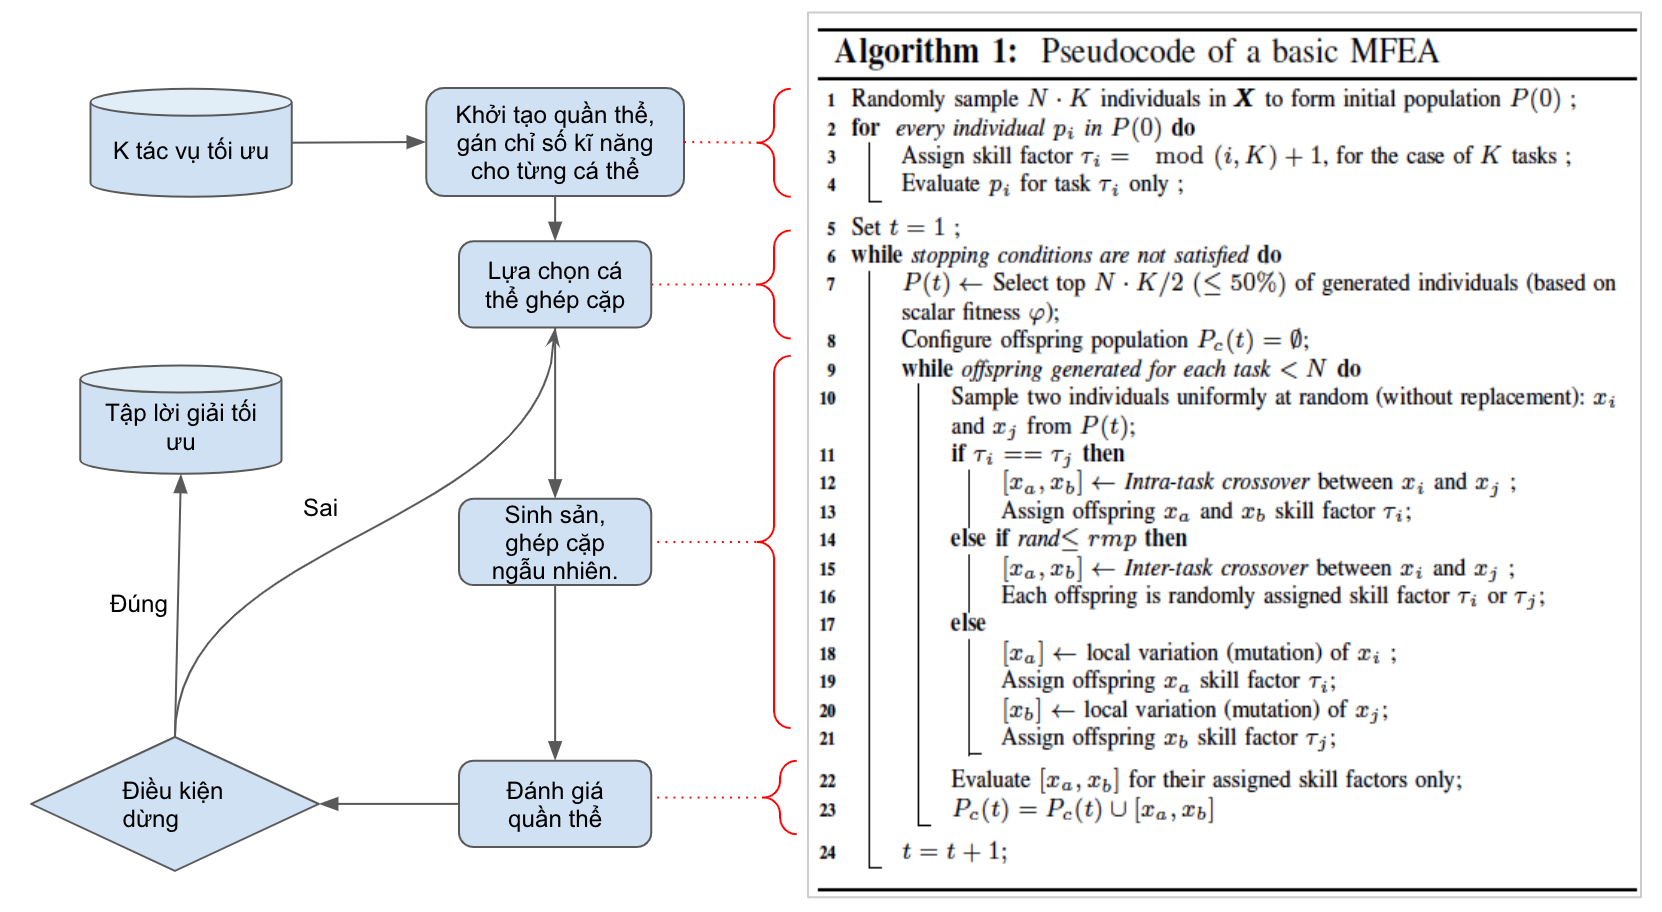
\includegraphics[width=0.85\linewidth]{thesis/images/mfea-alg.png}}
    \caption{Lược đồ giải thuật tiến hóa đa nhiệm MFEA-I \cite{gupta2016multifactorial}}
    \label{mfea-flow}
\end{figure}

Trong đó điểm khác biệt lớn nhất của MFEA-I so với thuật toán tiến hóa thông thường được mô tả tại \ref{section:cea} là cho phép lai ghép cá thể của các bài toán khác nhau theo một xác suất ghép cặp ngẫu nhiên (thuật ngữ gốc: \emph{random mating propability - rmp}). Phép lai ghép ngẫu nhiên đa nhiệm này đem đến một khả năng chia sẻ các gen tốt gữa các bài toán tối ưu hóa để đồng thời giải quyết cùng lúc chúng với tốc độ hội tụ nhanh hơn. 

Tuy nhiên, liệu việc kết hợp các lời giải của các bài toán tối ưu hóa khác nhau thì có sinh ra lời giải tốt hay không? Hoặc ít nhất cũng cần chỉ ra được trong trường hợp nào thì tốt, trường hợp nào thì không tốt. Các mục tiếp theo trong đồ án sẽ làm rõ hơn về vấn đề này.


\section{Tiến hóa đa nhiệm dưới góc độ xác suất}
\subsection{Mô hình hỗn hợp trong môi trường đa nhiệm}
Trong thống kê mô hình hỗn hợp (thuật ngữ gốc: \emph{mixture models}) là mô hình xác suất đại diện cho sự hiện diện của các quần thể con trong tổng thể \cite{rasmussen2000infinite}. Nói cách khác mô hình hỗn hợp là một hỗn hợp các phân phối xác suất đại diện cho các tập hợp con tạo thành quần thể.
\\[0.5cm]
\begin{figure}[h!]
    \centering
        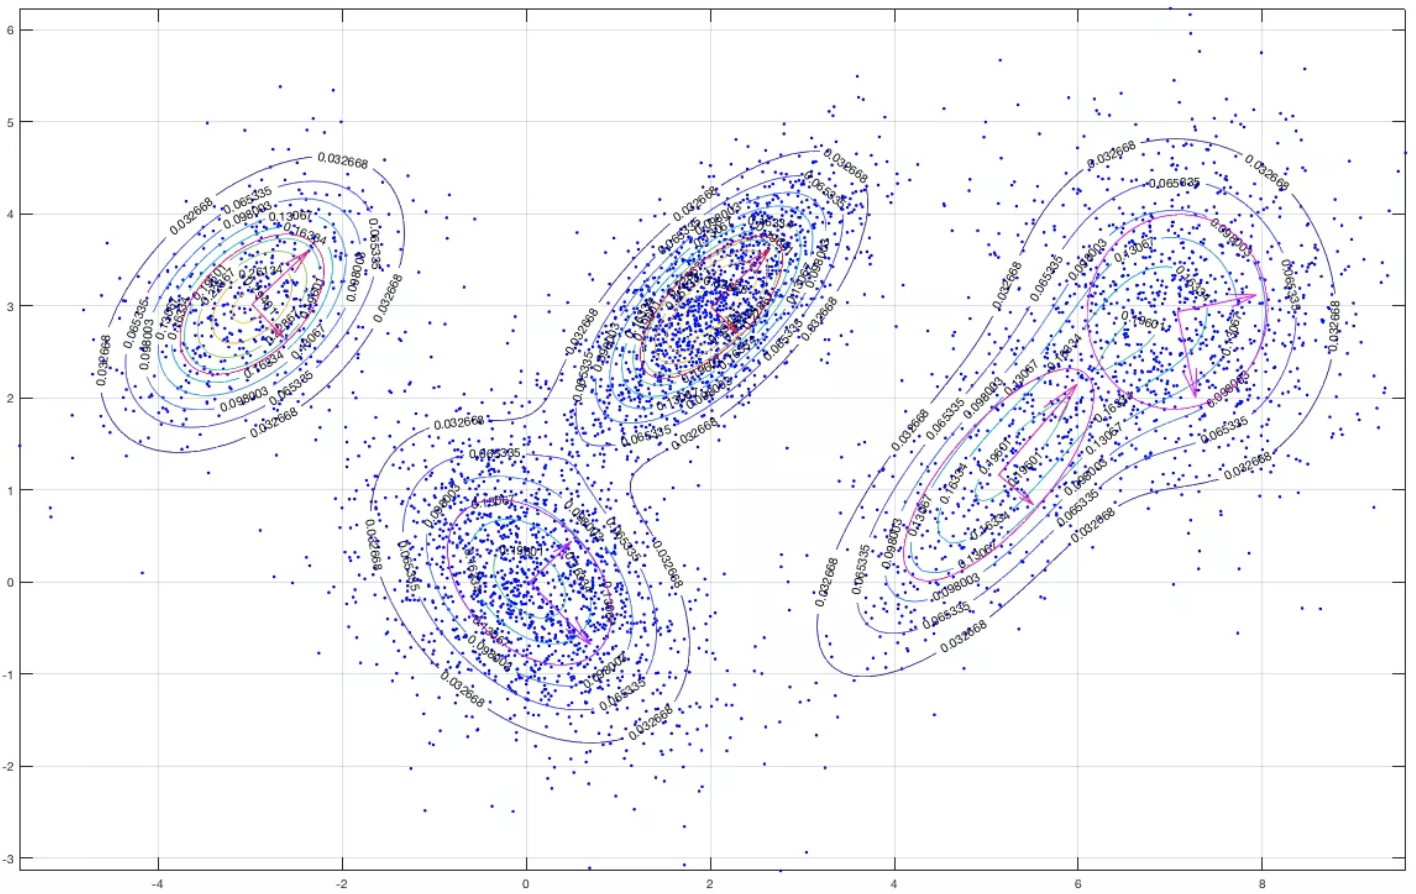
\includegraphics[width=9cm]{mixture-model.png}
    \caption{Ví dụ về mô hình hỗn hợp trong quần thể}
    \label{fig:mixture-model}
\end{figure}

Không làm mất tính tổng quát, ta coi $P^k$ là tập hợp các quần thể con liên kết với tác vụ thứ $k$ trong tập các tác vụ $k \in \{1,2,...K\}$. Hàm mục tiêu là $f_k$ và $f_k^* = f_k(x^*)$ là cực đại toàn cục tại tác vụ thứ $k$. Trong tiến hóa đa nhiệm, mỗi tác vụ các tác vụ tại một thế hệ thứ $t > 0$ có tập các quần thể con tương ứng với phân xác suất là $p^1(x,t), p^2(x,t),...., p^k(x,t)$. Sự tương tác giữa các tác vụ, quần thể con cái được sinh ra tại thế hệ thứ $t$ và bởi tác vụ thứ $k$ được biểu diễn dưới dạng một mô hình hỗn hợp như sau:
\begin{equation}
    q^k(x,t) = \alpha_k \cdot p^k(x,t) + \sum_{j \neq k} \alpha_j \cdot p^j(x,t)
    \label{equa:mixture_distribution}
\end{equation}
Ở đây phân phối $q^k(x,t)$ là một hỗn hợp $K$ phân phối với hệ số hỗn hợp là $\alpha^{'}s$. Có $\alpha_k + \sum_{j \neq k} \alpha_j = 1$ và $\alpha^{'}s >= 0$. 

Có thể thấy việc chia sẻ tri thức trong môi trường đa nhiệm là hệ quả của quá trình lấy mẫu các giải pháp phù hợp từ những phân phối hỗn hợp trong công thức \ref{equa:mixture_distribution}. Tuy nhiên trong trường hợp thiếu đi những tri thức tiên nghiệm về mối quan hệ giữa các tác vụ, việc chia sẻ tri thức có nguy cơ cao không những tri thức được chia sẻ không giúp các tác vụ tối ưu hóa nhanh hơn mà còn khiến nó bị giảm tốc độ. Hay nói cách khác là chia sẻ âm (thuật ngữ gốc: \emph{negative transfer}). Vậy vấn đề cần đặt ra là làm thế nào để xác định khi nào cần chia sẻ tri thức, khi nào không và mức độ chia sẻ là bao nhiêu. Điều này được thể hiện ở hệ số hỗn hợp $\alpha^{'}s$, giá trị $\alpha^{'}s$, và các hệ số này cần được học và tối ưu tại mỗi thế hệ sao cho phù hợp nhất với mối quan hệ giữa các tác vụ tại thời điểm đang xét.

Vậy thuật toán MFEA-I đã mô tả ở (\ref{mfeai}) với điểm nổi bật là khả năng chia sẻ tri thức giữa các tác vụ tối ưu khác nhau có gặp vấn đề negative transfer không? Dưới đây tôi sẽ đi vào phân tích thuật toán MFEA-I dưới một góc độ khác, góc độ xác suất để để trả lời cho câu hỏi đó.

\subsection{Phân tích tiến hóa đa nhiệm dưới góc độ xác suất}
Để dễ dàng phân tích thuật toán MFEA-I dưới góc độ xác suất thì không mất tính tổng quát, đưa ra một số giả thiết sau:
\begin{itemize}
    \item Toán tử sinh sản trong thuật toán MFEA-I tuân theo quy tắc xoay quanh cha mẹ (thuật ngữ gốc: \emph{parent-centric}), có nghĩa quần thể con được sinh ra có xác suất cao nằm gần với bố mẹ. 
    % Thực tế việc giả định này nhằm đơn giản việc phân tích, thay vì \emph{parent-centric} thì toán tử sinh sản ngẫu nhiên cũng sẽ có kết quả tương tự, tôi sẽ để phần chứng minh tại phụ lục bổ sung. 
    \item Phân phối xác suất của quần thể cha mẹ tuân theo phân phối chuẩn nhiều chiều.
    % với trung vị là $m$ và hiệp phương sai là $\sum$. Điều này dẫn đến hệ quả là phân phối của tập con cái sẽ rất gần với phân phối của tập cha mẹ: $p_c(x,t) \approx p(x,t)$. 
\end{itemize}
Giống như phần mô tả \emph{mô hình hỗn hợp trong môi trường đa nhiệm} ở trên, trong MFEA-I ta có thể định nghĩa lại như sau:
\begin{itemize}
    \item Tại thế hệ thứ $t$, cả $K$ tác vụ sẽ có quần thể chung là $P_t$
    \item Tại thế hệ thứ $t$ mỗi tác vụ thứ $k$ có tập quần thể con liên kết với nó là $P_t^k$
    \item $P_t$ được biểu diễn bởi mô hình $p(x,t)$, con cái của chúng được biểu diễn bởi $p_c(x,t)$
    \item $P_t^k$ được biểu diễn bởi mô hình $p^k(x,t)$, con cái của chúng được biểu diễn bởi $p_c^k(x,t)$
\end{itemize}
Tuân theo giả thiết về toán tử parent-centric, một ước lượng toàn bộ quần thể $p_c(x,t) \approx p(x,t)$. Tuy nhiên những cá thể con cái thuộc tác vụ $k$ được sinh ra do quá trình trao đổi chéo của bố mẹ là $p_c^k(x,t)$ thì \textbf{không nhất thiết phải tuân theo nguyên tắc này}.
Ta có mô hình hỗn hợp phân phối của tập con cái tại thế hệ thứ $t$ của tác vụ $k$ được biểu diễn bởi:
\begin{equation}
    p_c^k(x,t) = [1 - \frac{0.5 \cdot (K - 1) \cdot rmp}{K} ] \cdot p^k(x,t) + \sum_{j \neq k}\frac{0.5 \cdot rmp}{K} \cdot p^j(x,t).
    \label{equa:mfea_offstring_distribution}
\end{equation}
Trong đó các hệ số $\alpha_k$ và $\alpha_j$ của công thức \ref{equa:mixture_distribution} được thay thế lần lượt bởi $[1 - \frac{0.5 \cdot (K - 1) \cdot rmp}{K} ] $ và $\frac{0.5 \cdot rmp}{K}$. 
% Phần chứng minh các hệ số này tôi xin phép đặt tại phụ lục bổ sung. \emph{Phải chứng minh cái này}

Theo công thức \ref{equa:mfea_offstring_distribution}, có thể thấy hệ số hỗn hợp $\alpha$ phụ thuộc vào giá trị $rmp$. Tuy nhiên trong thuật toán MFEA-I thì hệ số $rmp$ là cố định dùng chung cho tất cả các cặp tác vụ được chọn ngay từ khi khởi tạo. Hệ số này càng lớn thì khả năng chia sẻ, khả năng trao đổi chéo khác tác vụ càng lớn  hoặc ngược lại khi hệ số này càng nhỏ thì việc chia sẻ, trao đổi tri thức gần như không xảy ra. Hay nói cách khác thuật toán MFEA-I sẽ trở về tương tự thuật toán đơn nhiệm thông thường mà không khai thác được mối quan hệ giữa các tác vụ. Tuy nhiên trong trường hợp cặp tác vụ không có sự bổ trợ lẫn nhau thì việc trao đổi là không cần thiết và còn khiến các tác vụ hội tụ chậm hơn so với thuật toán tiến hóa đơn nhiệm thông thường theo chứng minh của Bali, Ong, Gupta and Tan (dẫn chứng).
Với nguyên tắc này phân phối các cá thể mới của tác vụ được sinh ra $p_c^k(x,t)$ như trong công thức \ref{equa:mfea_offstring_distribution} sẽ cần phải càng gần với phân phối của cá thể cha mẹ $p^k(x,t)$ càng tốt (do đã quy định toán từ sinh sản là parent-centric). Hay nói cách khác hệ số hỗn hợp $\alpha_k >> \alpha_j$.
Nhìn vào công thức \ref{equa:mfea_offstring_distribution} thì để thực hiện điều này sẽ có 2 cách:
\begin{itemize}
    \item $rmp = 0$ : Nghĩa là không có sự trao đổi nào giữa các tác vụ, quần thể con cái sinh ra sẽ tuân theo quy luật parent-centric và phân phối của quần thể con cái sẽ gần với quần thể cha mẹ.
    \item $rmp > 0$ : Điều khiển hệ số $rmp$ để xác định và giảm tác động của việc trao đổi âm giữa các tác vụ.
\end{itemize}
Cách thứ nhất thực tế rất đơn giản vì chỉ cần xét $rmp = 0$ tuy nhiên cách này sẽ khiến ta không khai thác được khả năng của tiến hóa đa nhiệm, điểm tốt giữa sự trao đổi tri thức khác tác vụ. Vậy nên phần dưới đây tôi chỉ tập trung vào phương pháp thứ 2 là điều khiển giá trị của $rmp > 0$ để giảm tác động của việc trao đổi âm giữa các tác vụ.

Tuy nhiên, làm thế nào để ước lượng giá trị $rmp$ của từng cặp tác vụ tại từng thời thế hệ sao cho phù hợp với mối quan hệ giữa cặp tác vụ đó để ta đạt được hiệu quả trao đổi tri thức cao nhất? 

Đây cũng là ý tưởng chính mở ra hướng đi mới cho tiến hóa đa nhiệm - thuật toán tiến hóa đa nhiệm với ước lượng hệ số trao đổi $rmp$ trực tuyến, và đây cũng là hướng đi chính cho các giải thuật đề xuất trong đồ án này.

\section{Tiến hóa đa nhiệm với ước lượng hệ số trao đổi trực tuyến}
\label{section:mfeaii}
\subsection{Ý tưởng xây dựng thuật toán}
\label{section:idea}
\subsection{Xây dựng ma trận xác suất ghép cặp ngẫu nhiên $RMP$}

Trong thuật toán MFEA-I thông thường $rmp$ là một giá trị vô hướng biểu diễn chung cho xác suất giao phối ngẫu nhiên giữa các tác vụ, tuy nhiên thực tế thì mỗi cặp tác vụ lại có một mức độ tương quan riêng. Bởi vậy dẫn đến một ý tưởng đó là xây dựng xác suất ghép cặp ngẫu nhiên $rmp$ dưới dạng một ma trận xác suất ghép cặp ngẫu nhiên đối xứng $RMP$ như sau:
\begin{equation}
    RMP =
    \begin{bmatrix}
        rmp_{1,1} & rmp_{1,2} & \cdot & \cdot \\
        rmp_{2,1} & rmp_{2,2} & \cdot & \cdot \\
        \cdot & \cdot & rmp_{j,j} & \cdot \\
        \cdot & \cdot & \cdot & \cdot \\
    \end{bmatrix}
\end{equation}
Trong đó $rmp_{j,k} = rmp_{k,j}$ là hệ số trao đổi giữa tác vụ $j$ và tác vụ $k$, thêm nữa có $rmp_{j,j} = 1$ $\forall j$. 
\subsection{Ước lượng phân phối của các quần thể con}
Tại thời điểm $t$ xem xét phân phối $g^k(x,t)$ là mô hình ước lượng của phân phối chuẩn $p^k(x,t)$ của tác vụ thứ $k$, $g^k(x,t)$ được xây dựng từ tập nhỏ dân số $P^k(t)$. Bằng việc thay thế hàm mật độ của phân phối chuẩn và sử dụng phần tử trong ma trận $RMP$ thay vì giá trị $rmp$ vô hướng ta có phân phối tập con cái được sinh ra như sau:
\begin{equation}
    g_c^k(x,t) = [1 - \frac{0.5}{K}\cdot \sum_{k \neq j}rmp_{k,j}] \cdot g^k(x,t) + \frac{0.5}{K} \sum_{j \neq k} rmp_{k,j} \cdot g^j(x,t).
    \label{equa:true_distribution}
\end{equation}
Với $g_c^k(x,t)$ là mô hình xác suất hỗn hợp ước lượng gần đúng cho quần thể con cái $p_c^k(x,t)$. Như đã trình bày ở trên, để giảm tác động của trao đổi âm giữa các tác vụ thì cần đưa phân phối $p_c(x,t)$ càng gần với phân phối của quần thể $p(x,t)$ càng tốt. Điều này có nghĩa rằng ta học tham số $rmp$ sao cho phân phối hỗn hợp $g_c^k(x,t)$ sao cho nó xấp xỉ với $p^k(x,t)$ trên tập tất cả tác vụ $k \in {1,2,...K}$.

\subsection{Học trực tuyến ma trận RMP}
    \label{sub:rmp-learning}
    Mỗi tác vụ thứ $k$ sẽ tương ứng với một tập cá thể của chúng là $P^k(t)$, tập này tuân theo phân phối $g^k(x,t)$. Và giả sử tại mỗi thế hệ thì trong tập $P^k(t)$ sẽ bao gồm $N/2$ cá thể là cá thể cha mẹ được truyền từ thế hệ trước sang thế hệ này.
    Cùng với đó theo ý tưởng đã trình bày ở phần \ref{section:idea}, ma trận $RMP$ là tham số của mô hình phân phối xác suất hỗn hợp $g_c^k(x,t)$ với $k \in {1,2,...K}$. Một ý tưởng tự nhiên là để $g_c^k(x,t) \approx p^k(x,t)$ thì phân phối $g_c^k(x,t)$ cũng sẽ phù hợp với tập các cá thể của thế hệ hiện tại và các cá thể này sẽ tuân theo phân phối $g_c^k(x,t)$. Vậy bài toán trở thành tối ưu ma trận $RMP$ sao cho cực đại hóa giá trị hàm maximum log-likelihood:
    \begin{equation}
        \max_{RMP}\sum_{k=1}^{K}\sum_{i=1}^{N/2}\log{g_c^k(x_{ik},t)}
        \label{equa:likelihood}
    \end{equation}
    với $x_{ik}$ là cá thể thứ $i$ trong tập $P^k(t)$.
    
    Nhưng liệu khi học ma trận $RMP$ sao cho phân phối $g_c^k(x,t)$ phù hợp với tập các cá thể của thế hệ hiện tại $\forall k \in {1,2,...K}$, thì có kéo theo $g_c^k(x,t)$ trở lên gần với $p^k(x,t)$? Để xác định xem 2 phân phối có thực sự gần nhau hay không thì có một phương pháp thông dụng đó là sử dụng phương pháp phân kỳ Kullback-Leiber (thuật ngữ gốc: \emph{Kullback-Leiber divergence - KL}) \cite{hershey2007approximating}. Một cách cụ thể $KL$ sẽ tính toán lượng thông tin bị mất mát khi hàm mật độ $g$ được sử dụng để ước lượng hàm mật độ $p$. Điều này thể hiện tương đương mức độ gần nhau giữa 2 phân phối.
    Cụ thể $KL$ giữa 2 phân phối $p$ và $g$ được định nghĩa như sau:
    \begin{equation}
        KL(p\Vert g) = \int_{X}p(x)\cdot [log(x) - log(x)]\cdot\,dx
        \label{equa:KL}
    \end{equation}
    Từ suy nghĩ này việc tối ưu sao cho $g_c^k(x,t)$ trở lên gần với $p^k(x,t)$ cũng sẽ tương đương việc tả tối thiểu hóa $KL$ giữa 2 phân phối. Và qua công thức \ref{equa:likelihood} và \ref{equa:KL}, Bali, Ong, Gupta and Tan qua một số biến đổi đơn giản đã chứng minh khi tối đa hóa maximum log-likelihood \ref{equa:likelihood} \cite{white1982maximum} thì cũng sẽ tương đương với việc tối thiểu hóa hàm khoảng cách $KL$ giữa 2 phân phối $p$ và $g$. Hay phân phối $g_c^k(x,t)$ sẽ gần hơn với $p^k(x,t)$ sau quá trình học trực tuyến ma trận $RMP$.
    \begin{equation}
        \text{công thức } \ref{equa:likelihood} \Leftrightarrow \min_{RMP}\sum_{k=1}^{K}KL(p^k(x,t)\|g_c^k(x,t))
        \label{equa:KL}
    \end{equation}
\subsection{Cấu trúc thuật toán}
    Biểu diễn thuật toán qua các bước:
    \begin{figure}[ht]
        \centering
        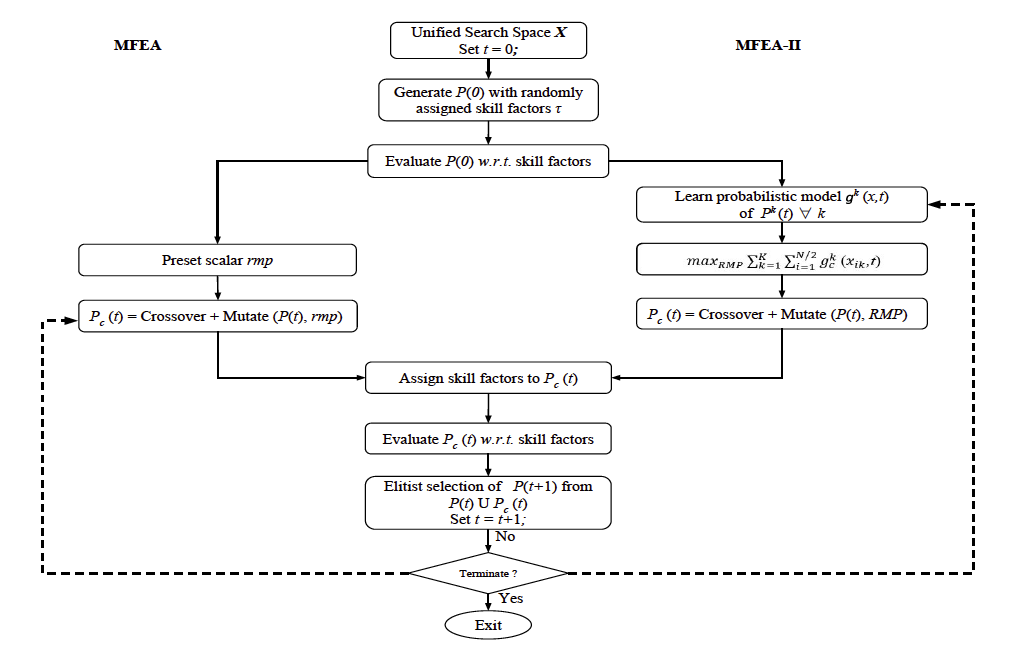
\includegraphics[width=15cm,height=12cm]{mfeaii.png}
        \caption{Lược đồ so sánh các bước thực hiện giải thuật MFEA-I và MFEA-II. Nguồn \cite{bali2019multifactorial}}.
        \label{fig:mfeaii}
    \end{figure}
    Hình \ref{fig:mfeaii} mô tả một góc nhìn tổng quan về sự khác biệt giữa MFEA và MFEA-II. Trong đó có thể chia 2 thuật toán này làm 3 pha chính theo thứ tự từ trên xuống: khởi tạo, trao đổi chéo, đánh giá và lựa chọn. Dễ thấy sự giống nhau nằm ở pha đầu tiên và cuối cùng. Điểm khác biệt của MFEA-II trong phá thứ 2 bởi quá trình học trực tuyến ma trận $RMP$ với phương pháp đã được trình bày ở mục \ref{sub:rmp-learning}. Mô tả quá trình học trực tuyến ma trận $RMP$ dưới dạng mã giả trong thuật toán \ref{alg:online-rmp-learning}
    \begin{algorithm}[ht]
        \caption{Học trực tuyến ma trận $RMP$}
        \begin{algorithmic}[1]
            \State Xây dựng một mô hình phân phối ước lượng $g^k(x,t)$ trên mỗi tập cá thể $P^k(t)$. $\forall k \in {1,2,...K}$
            \State Tối ưu hóa mô hình hỗn hợp $\max_{RMP}\sum_{k=1}^{K}\sum_{i=1}^{N/2}\log{g_c^k(x_{ik},t)}$
        \end{algorithmic}
        \label{alg:online-rmp-learning}
    \end{algorithm} \\
    Pha trao đổi khác tác vụ sẽ được mô tả trong thuật toán 5, khi các giải pháp được trao đổi giữa các tác vụ sẽ phụ thuộc vào ma trận $RMP$ đã học ở thuật toán \ref{alg:inter-task crossover}. Trong trường hợp ma trận $RMP$ học được toàn giá trị $0$ thì MFEA-II sẽ hoạt động tương tự với thuật toán tiến hóa kinh điển trong việc học song song từng tác vụ đơn lẻ. \\ 
    \begin{algorithm}[h!]
        \caption{Trao đổi khác tác vụ trong MFEA-II}
        \begin{algorithmic}[1]
            \State Chọn 2 cá thể ngẫu nhiên $x_i$ và $x_j$ từ quần thể $P(t)$:
            \If {$(\tau_i  \neq \tau_j)$}
                \If {$rand \leq rmp_{\tau_i,\tau_j}$}
                    \State $[x_a, x_b]$ $\leftarrow$ \emph{Trao đổi khác tác vụ} giữa $x_i$ và $x_j$;
                    \State Mỗi cá thể con cái sinh ra sẽ được gán ngẫu nhiên một giá trị thuộc tính kĩ năng $\tau_i$  hoặc $\tau_j$;
                \Else 
                    \State Lựa chọn ngẫu nhiên $x_i^{'}$ với thuộc tính kĩ năng $\tau_i$;
                    \State $[x_a]$ $\leftarrow$ \emph{Trao đổi cùng tác vụ} giữa $x_i$ và $x_i^{'}$;
                    \State Gán cá thể con cái $x_a$ với thuộc tính kĩ năng $\tau_i$;
                    \State Lựa chọn ngẫu nhiên $x_j^{'}$ với thuộc tính kĩ năng $\tau_j$;
                    \State $[x_b]$ $\leftarrow$ \emph{Trao đổi cùng tác vụ} giữa $x_i$ và $x_i^{'}$;
                    \State Gán cá thể con cái $x_b$ với thuộc tính kĩ năng $\tau_j$;
                
        \end{algorithmic}
        \label{alg:inter-task crossover}
    \end{algorithm}
     Tuy nhiên tại sao lại sử dụng MFEA-II để huấn luyện mạng neural trong khi các thuật toán huấn luyện mạng neural kinh điển sử dụng phương pháp gradient-based vẫn đang được hầu hết các nhóm nghiên cứu sử dụng. Trong chương tiếp theo, đồ án sẽ trình bày các yêu cầu cấp thiết của việc áp dụng này và qua đó là đề xuất, giải thuật áp dụng chi tiết.
    